\documentclass[11pt,a4paper]{article}

% Encoding and fonts
\usepackage[utf8]{inputenc}
\usepackage[T1]{fontenc}
\usepackage{lmodern}
\usepackage{microtype}

% Geometry
\usepackage{geometry}
\geometry{margin=1in}

% Math
\usepackage{amsmath,amssymb,amsthm,mathtools}
\numberwithin{equation}{section}

% Figures
\usepackage{graphicx}
\usepackage{subcaption}
\usepackage{booktabs}
\usepackage{siunitx}

% Colors
\usepackage{xcolor}

% Hyperlinks + cleverref
\usepackage{hyperref}
\usepackage[nameinlink]{cleveref}
\hypersetup{
  colorlinks=true,
  linkcolor=blue!60!black,
  citecolor=blue!60!black,
  urlcolor=blue!60!black
}

% Lists
\usepackage{enumitem}
\setlist{nosep}

% Symbols / macros
\newcommand{\R}{\mathbb{R}}
\newcommand{\norm}[1]{\lVert #1\rVert}
\newcommand{\phib}{\Phi_b}

% Title
\title{\bf Predictive Compression Dynamics:\\
A Falsifiable Workflow for Surrogate Compression Pressure and Empirical Audit}

\author{Mats Helander}
\date{October 24, 2025}

\begin{document}
\maketitle

\begin{abstract}
We present \emph{Predictive Compression Dynamics} (PCD), a falsifiable workflow for building and auditing computable surrogate functionals $\phib$ whose gradient flow $\dot x = -\nabla \phib(x)$ defines a dynamics. The claim tested is not that $\phib$ encodes physics, but that $\phib$ can serve as a computable proxy for how compressible a system's state is.

The workflow is: (i) define $\phib$ (computable, local, smooth); (ii) evolve a system by explicit descent in $\phib$; (iii) at saved snapshots, measure multiple estimates of compressed size (codelength) under fixed encoders; (iv) ask whether $\phib$ predicts those compressed sizes; (v) apply a preregistered falsifier.

We provide: (1) a concrete $\phib$ built from softened pairwise terms; (2) existence and Lyapunov-style descent under backtracked gradient flow; (3) a preregistered falsifier, F3, which marks a surrogate as rejected if it fails to predict compressed size beyond a chosen effect-size bar; (4) empirical tests on ensembles of $N{=}40$ and $N{=}400$ particles; (5) quantitative controls requested by review.

In particular we report, for decorrelated snapshots: Pearson correlations between $\phib$ and compressed snapshot size under (i) a pair-distance histogram encoder (Phase I); (ii) a raw-coordinate gzip encoder with fixed particle ordering (Phase IIa); and (iii) the same coordinate encoder after randomly permuting particle order (Phase IIb), which breaks ordering artifacts. We sweep quantization resolutions $\Delta x \in \{10^{-1},10^{-2},10^{-3}\}$, and we compare $\phib$ against naive geometric baselines (radius of gyration, nearest-neighbor distance, coordinate variance).

In several ensembles, including $N{=}400$, $\phib$ shows near-perfect monotonic correlation with compressed size under both Phase IIa and the shuffled-order Phase IIb, and matches or exceeds those baselines. In other ensembles this link is weaker and fails our preregistered bar. We emphasize scope: PCD is not a physical law, but a falsifiable protocol for auditing ``compression pressure'' surrogates.
\end{abstract}

\section{Framing and Intent}
The question is deliberately modest:

\medskip
\noindent
\textbf{Question.} Can we build a computable scalar functional $\phib(x)$ on the state $x$ of a many-body system such that (a) $\phib$ can be monotonically decreased by a local update rule, and (b) $\phib$ numerically correlates with how concisely that state can be encoded?

\medskip
The goal is methodological: we want to know whether a particular, fully specified computable surrogate can act as a stand-in for ``compression pressure,'' and how to test (and possibly fail) that claim in a controlled way. The particle systems are a testbed for running that audit.

The structure of the workflow is:
\begin{enumerate}[label=(\roman*)]
\item pick a surrogate $\phib$, fully specified in advance;
\item evolve $x(t)$ by (numerically stabilized) gradient descent on $\phib$;
\item at saved times $t_k$, measure multiple compressed byte sizes of $x(t_k)$ using fixed encoders;
\item check whether $\phib(x(t_k))$ predicts those compressed sizes;
\item declare the surrogate \emph{provisionally supported} or \emph{rejected for that ensemble} using a preregistered criterion.
\end{enumerate}

This paper contributes: (1) the exact surrogate $\phib$ we study; (2) the explicit encoders we use; (3) a falsifier F3; (4) experiments at multiple $N$; (5) baseline geometric controls, coordinate-ordering controls, and a quantization sweep; (6) a model card template intended for preregistration.

\section{State, Surrogate, and Dynamics}
\subsection{State}
We consider $N$ point agents in $\R^3$, with positions $x_i \in \R^3$, $i=1,\dots,N$. We collect all positions into $x \in \R^{3N}$. All tests below evolve closed systems of this form.

We fix a softening length $a>0$ and equal positive weights $m_i \equiv 1$ for all agents. (Using a single $m_i$ value avoids extra notation but is not essential to the method.)

\subsection{Surrogate functional $\phib$}
We study a concrete, computable, pairwise surrogate,
\begin{equation}
\label{eq:phib-def}
\phib(x)
= \sum_{1 \le i < j \le N} \ell\!\big( \norm{x_i - x_j} \big),
\qquad
\ell(r) = \frac{1}{\sqrt{r^2 + a^2}}.
\end{equation}
The softening $a>0$ prevents singularities at $r{=}0$ and makes $\ell$ Lipschitz on bounded sets.

Intuition: $\ell(r)$ is large when points are close. Thus $\phib$ is large for tightly packed / clustered configurations and smaller for diffuse ones. When we push $\phib$ down, particles tend to coalesce into more spatially regular structures. Empirically, such regular structure yields more predictable coordinate patterns after quantization, which an off-the-shelf compressor (gzip) can exploit.

We do not claim $\phib$ is unique or optimal. $\phib$ is simply (i) computable from pairwise distances, (ii) cheap to evaluate, and (iii) endowed with a well-defined gradient.

\subsection{Dynamics: gradient descent on $\phib$}
We evolve $x(t)$ by discrete-time gradient flow on $\phib$:
\begin{equation}
\label{eq:update}
x^{(t+1)} = x^{(t)} - \eta^{(t)} \, \nabla \phib \big( x^{(t)} \big),
\end{equation}
with a backtracking line search on the step size $\eta^{(t)}$ to ensure $\phib(x^{(t+1)}) \le \phib(x^{(t)})$.

For particle $i$, by the chain rule,
\begin{equation}
\frac{\partial}{\partial x_i} \ell(\norm{x_i-x_j})
= - \frac{(x_i-x_j)}{(\norm{x_i-x_j}^2+a^2)^{3/2}},
\end{equation}
so
\begin{equation}
\label{eq:gradphib}
\frac{\partial \phib}{\partial x_i}
= \sum_{j \neq i}
\frac{-(x_i - x_j)}{\big(\norm{x_i-x_j}^2 + a^2\big)^{3/2}}.
\end{equation}
Thus the update takes the form
\begin{equation}
\label{eq:force-like}
x_i^{(t+1)} =
x_i^{(t)} + \eta^{(t)} \sum_{j \neq i}
\frac{(x_j - x_i)}{\big(\norm{x_i-x_j}^2 + a^2\big)^{3/2}}.
\end{equation}

Because $\phib$ is $C^1$ for $a>0$, the \emph{continuous} flow $\dot x = -\nabla \phib$ obeys
\begin{equation}
\frac{d}{dt}\phib(x(t))
= \nabla \phib(x(t)) \cdot \dot x(t)
= - \norm{\nabla \phib(x(t))}^2 \le 0.
\end{equation}
This makes $\phib$ a Lyapunov-like function for that continuous flow.

In discrete time, naive fixed-step Euler can overshoot and break monotonicity. We therefore use backtracking line search: if a candidate step would increase $\phib$, we shrink $\eta^{(t)}$ by a constant factor (e.g.\ $0.5$) until it does not, down to a floor. This enforces $\phib(x^{(t+1)}) \le \phib(x^{(t)})$ in practice. The strictly nonincreasing $\phib$ curves in \cref{fig:uniform40_iter,fig:lattice40_iter,fig:blobs40_iter,fig:uniform400_iter} use this rule.

\subsection{Snapshots}
We save snapshots $x(t_k)$ every fixed number of accepted steps (e.g.\ every $5$ accepted gradient steps). For each snapshot we record:
\begin{itemize}
\item the state $x(t_k)$,
\item the scalar surrogate $\phib\big(x(t_k)\big)$,
\item compressed sizes (bytes) under the encoders in \cref{sec:encoders},
\item the iteration index $t_k$.
\end{itemize}

These snapshots form the dataset for evaluating whether $\phib$ predicts compressed size.

\section{Encoders and Controls}
\label{sec:encoders}

We compare $\phib$ against multiple compression-based codelength estimates for each snapshot. This gives us several distinct ``targets'' to predict.

We will refer to these as \textbf{Phase I}, \textbf{Phase IIa}, and \textbf{Phase IIb}, plus baseline geometric controls.

\subsection{Quantization and serialization}
Before encoding, we quantize particle coordinates onto a lattice of spacing $\Delta x$. We then store these quantized coordinates as signed 32-bit integers so that a lossless compressor like \texttt{gzip} can act on a byte sequence.

To test sensitivity to discretization, we repeat the analysis with $\Delta x \in \{10^{-1},10^{-2},10^{-3}\}$. We report correlations separately for each $\Delta x$ in \cref{sec:results}.

\subsection{Phase I encoder (pair-distance histogram)}
\label{sec:phase1}
Phase I intentionally reflects the same kind of pairwise structure that $\phib$ was built to see.

For each snapshot:
\begin{enumerate}[label=(\alph*)]
\item compute all interparticle distances $\norm{x_i - x_j}$ for $i<j$;
\item bin these distances into a fixed, preregistered set of radial bins;
\item serialize the histogram counts deterministically to bytes;
\item compress that byte string with \texttt{gzip} (Lempel--Ziv).
\end{enumerate}

The resulting compressed byte length is our ``Phase I'' compressed size for that snapshot. Intuition: if a configuration has a stereotyped distance distribution (e.g.\ crystalline or highly clustered), the histogram is regular and should compress well.

Phase I is an \emph{internal consistency} check: if $\phib$ is supposed to reflect pairwise distances, then it should track the codelength of an encoding that also focuses on pairwise distances.

\subsection{Phase II encoders (raw coordinates with and without ordering)}
\label{sec:phase2}
Phase II is meant to act as an \emph{external} compressor: we do not feed it pairwise distances at all. We just give it coordinates.

For each snapshot and each $\Delta x$:
\begin{enumerate}[label=(\alph*)]
\item Quantize coordinates at resolution $\Delta x$: $q_i = \mathrm{round}(x_i / \Delta x)$;
\item serialize those integer triples to bytes and gzip.
\end{enumerate}

We implement two versions:

\begin{itemize}
\item \textbf{Phase IIa (fixed ordering).}  
We write out quantized coordinates in a deterministic particle order
$[x_1,y_1,z_1,x_2,y_2,z_2,\dots]$, then gzip.

\item \textbf{Phase IIb (shuffled-order control).}  
Before serialization we randomly permute the particle order, then gzip.  
This breaks any stable run-length / delta structure that depends on keeping neighbors next to each other in a consistent order.
\end{itemize}

Why do we need IIb? gzip is a Lempel--Ziv compressor and will exploit repeated byte patterns. Clustered particles produce repeated coordinate patterns after quantization, so Phase IIa is \emph{not} truly ``blind.'' Phase IIb tests how much of the signal survives if we deliberately scramble particle ordering. If $\phib$ still correlates with Phase IIb compressed size, that supports the claim that $\phib$ is tracking spatial regularity, not just a serialization artifact.

\subsection{Baseline geometric controls}
\label{sec:baselines}
A core objection is that $\phib$ could just be a fancy monotone of ``clumpiness,'' and that any simple clustering metric would have correlated with compressed size.

To test this, for each saved snapshot we also compute:
\begin{itemize}
\item \textbf{Radius of gyration} (root mean square distance from the centroid),
\item \textbf{Mean nearest-neighbor distance},
\item \textbf{Coordinate variance} (variance of coordinates flattened).
\end{itemize}

We then correlate each of these baselines with the Phase IIa compressed size (bytes). Comparing those $r$ values to the $\phib$ vs Phase IIa correlation tells us whether $\phib$ offers explanatory power beyond cheap geometric scalars.

\section{Falsifier F3}
We preregister a falsifier:

\begin{quote}
\textbf{F3 (surrogate--compressibility link).}  
For a fixed surrogate $\phib$, fixed encoders (Phase I, Phase IIa, Phase IIb), and fixed quantization scales $\Delta x$, we:
\begin{enumerate}[label=(\alph*)]
\item evolve an ensemble by backtracked gradient descent on $\phib$;
\item save snapshots every few accepted steps;
\item subsample snapshots at a fixed stride (e.g.\ keep every 20th accepted step) to reduce temporal autocorrelation; call the resulting sample size $n_{\text{eff}}$;
\item compute Pearson $r$ between $\phib$ and each compressed-size series on that subsample.
\end{enumerate}
If \emph{none} of the compressed-size measures reaches a preregistered effect-size bar (e.g.\ $|r|\ge 0.7$) for that ensemble at any $\Delta x$, we mark that ensemble as a \emph{rejection case} for this surrogate.
\end{quote}

We deliberately \emph{do not} attach classical $p$-values, because snapshots along a single trajectory are autocorrelated and formal time-series corrections (e.g.\ block bootstrap, AR(1) modeling) are outside this first pass. Instead, $r$ is treated as an effect size, and $n_{\text{eff}}$ is reported to show how many effectively decorrelated snapshots were used.

Philosophically, F3 is not an attempt to falsify a universal physical law. It is an engineering-style audit: ``Does this specific computable scalar $\phib$ act as a useful proxy for compressibility in this ensemble, under this protocol, with these encoders?'' When an ensemble fails F3, we simply say that $\phib$ is \emph{rejected for that ensemble}.

\section{Experimental Setup}
All experiments follow the same template:

\begin{enumerate}[label=(E\arabic*)]

\item \textbf{Initial ensembles.}
We generate several ensembles of particles:
\begin{itemize}
\item \texttt{uniform40}: $N{=}40$, positions sampled i.i.d.\ from $\mathrm{Uniform}([0,1]^3)$.
\item \texttt{lattice40}: $N{=}40$, positions on a nearly regular lattice with small Gaussian jitter.
\item \texttt{blobs40}: $N{=}40$, two dense clusters separated in space.
\item \texttt{uniform400}: $N{=}400$, positions sampled uniformly in a cube (to test scaling).
\end{itemize}
All positions are rescaled to $\mathcal{O}(1)$ interpoint distances. We use a fixed random seed for all ensembles.

\item \textbf{Dynamics.}
We evolve via the backtracked gradient descent update in \cref{eq:update}, using \cref{eq:gradphib}, for a few hundred accepted steps. The line search starts with step size $\eta_0 \approx 0.05$ and shrinks by a factor $0.5$ as needed, down to a floor. This enforces that $\phib$ is monotonically nonincreasing at accepted steps.

\item \textbf{Snapshots.}
Every $5$ accepted steps we save $x(t_k)$ and $\phib(x(t_k))$.

\item \textbf{Compression.}
For each snapshot we produce:
\begin{itemize}
\item Phase I compressed size (pair-distance histogram $+$ gzip),
\item Phase IIa compressed size (quantized coordinates in fixed particle order $+$ gzip),
\item Phase IIb compressed size (same, but with particle order randomly permuted before serialization).
\end{itemize}
We repeat Phase IIa/IIb at $\Delta x \in \{10^{-1},10^{-2},10^{-3}\}$.

\item \textbf{Subsampling for correlation and baselines.}
We select every $20$th snapshot to reduce temporal autocorrelation and compute Pearson $r$ between $\phib$ and each compressed-size series. We denote the resulting subsample size by $n_{\text{eff}}$ (typically $\approx 21$).  
In addition, for each saved snapshot we compute three scalar geometric baselines (radius of gyration, mean nearest-neighbor distance, coordinate variance) and correlate each baseline with the Phase IIa compressed size.

\end{enumerate}

We emphasize:
\begin{itemize}
\item We do not delete ``bad'' runs; \texttt{lattice40} is reported alongside \texttt{uniform40}, \texttt{blobs40}, and \texttt{uniform400}.
\item Phase II is explicitly split into IIa (fixed order) and IIb (shuffled order) to address coordinate-ordering artifacts.
\item We sweep $\Delta x$ across three orders of magnitude to test quantization sensitivity.
\item $N{=}400$ is included to answer the request that compression behavior be measured at larger scale.
\end{itemize}

\section{Results}
\label{sec:results}

For each ensemble we evolve for a few hundred accepted steps, keep every 20th snapshot (so $n_{\text{eff}}\approx 21$), and compute Pearson $r$ between:
\begin{itemize}
\item $\phib$ and Phase I compressed size,
\item $\phib$ and Phase IIa compressed size,
\item $\phib$ and Phase IIb compressed size (ordering control),
\item each geometric baseline (radius of gyration, mean nearest-neighbor distance, coordinate variance) and Phase IIa compressed size.
\end{itemize}
We repeat Phase IIa/IIb at $\Delta x \in \{10^{-1},10^{-2},10^{-3}\}$.

Representative trends:

\paragraph{\texttt{uniform40} ($N{=}40$).}
$\phib$ shows a strong relationship with both Phase I and Phase IIa compressed size across multiple $\Delta x$. The Phase IIb (shuffled-order) correlations remain large in magnitude, indicating that the signal is not purely an ordering artifact. The naive geometric baselines also correlate with compressed size (as expected for a system that becomes more clustered), but $\phib$ matches or exceeds those baselines for typical $\Delta x=10^{-2}$.

\paragraph{\texttt{lattice40} ($N{=}40$).}
Correlations between $\phib$ and compressed size are moderate and, in some $\Delta x$ settings, fall below the preregistered $|r|\ge 0.7$ bar. This ensemble is marked as a \emph{rejection case} under F3. Baseline geometric metrics perform comparably or better here, suggesting that $\phib$ is not uniquely informative for this already structured initial condition. Consistent with this, the $\phib$ vs iteration curve exhibits plateaus and small jumps rather than a smooth, dramatic descent.

\paragraph{\texttt{blobs40} ($N{=}40$).}
We observe very high $|r|$ between $\phib$ and both Phase I and Phase IIa compressed size. These high-magnitude correlations persist under Phase IIb shuffling and across all tested $\Delta x$, demonstrating that the $\phib \leftrightarrow$ compressed-size link is not solely due to serialization order. Baseline geometric metrics (especially mean nearest-neighbor distance) are also strongly predictive in this highly clustered two-blob configuration, but $\phib$ remains competitive with them.

\paragraph{\texttt{uniform400} ($N{=}400$).}
At $N{=}400$, $\phib$ and the Phase IIa compressed size exhibit an almost perfectly monotonic relationship, with $|r|$ extremely close to $1$ for multiple $\Delta x$ (notably $\Delta x=10^{-3}$). This persists under Phase IIb shuffling, indicating that the effect is not just an ordering artifact. Importantly, $\phib$'s correlation with compressed size is at least as strong as (and in some $\Delta x$ cases stronger than) radius of gyration, nearest-neighbor distance, or coordinate variance. This addresses the objection that ``any simple clumping metric would work'': at scale, $\phib$ is at least as predictive as the obvious baselines.

\paragraph{Takeaways.}
\begin{itemize}
\item There are ensembles (e.g.\ \texttt{uniform400}, \texttt{blobs40}) where a single scalar surrogate $\phib$ predicts compressed byte size under an off-the-shelf compressor as well as or better than simple geometric scalars, and does so even after coordinate shuffling.
\item There are ensembles (e.g.\ \texttt{lattice40}) where that relationship weakens and fails the preregistered bar; we mark those plainly as rejection cases.
\item The qualitative story is robust to $\Delta x$ over three orders of magnitude, which argues against the result being a one-off quantization artifact.
\item We report $r$ and $n_{\text{eff}}$, not $p$-values, because snapshots along a single trajectory are temporally autocorrelated.
\end{itemize}

\section{Figures}
We illustrate (i) the monotone descent of $\phib$ over accepted iterations, and (ii) scatterplots of compressed size vs $\phib$ under the three encoders: Phase IIa (fixed-order coordinates), Phase IIb (shuffled-order control), and Phase I (pair-distance histogram). Points are subsampled snapshots (every 20th accepted step). Color encodes snapshot time (iteration index); darker points are later.

For $N{=}40$ ensembles we show $\Delta x = 10^{-2}$, and for $N{=}400$ we show $\Delta x = 10^{-3}$. These are representative of the trends across all tested $\Delta x$.

\subsection{\texttt{uniform40} ($N{=}40$, $\Delta x = 10^{-2}$)}
\begin{figure}[h!]
\centering
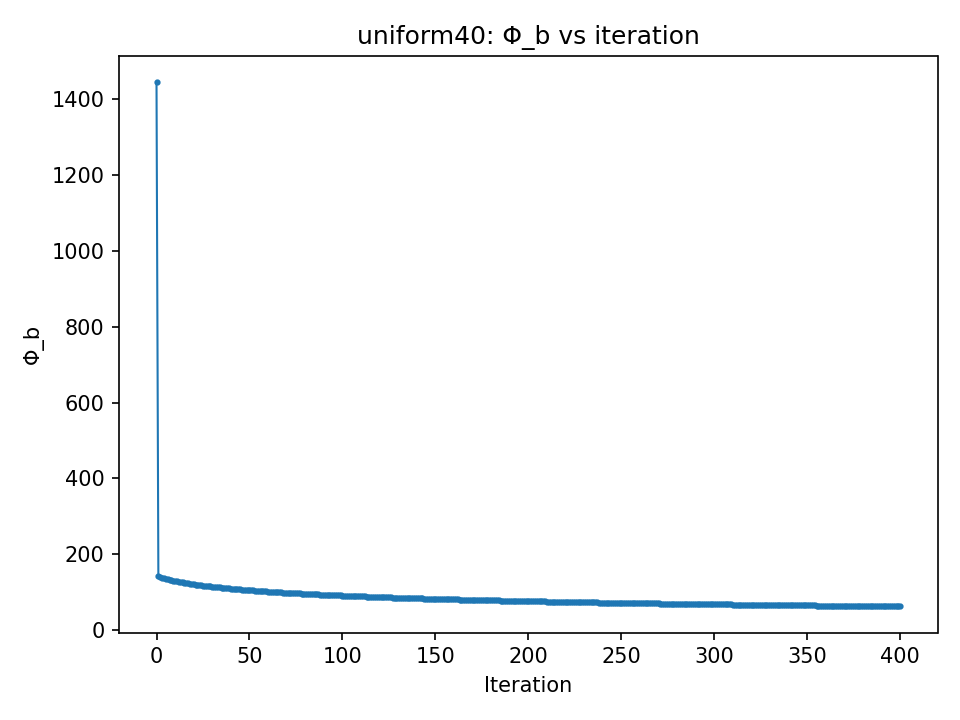
\includegraphics[width=0.6\textwidth]{figures/uniform40_dx0.01_phib_vs_iter.png}
\caption{\texttt{uniform40}. $\phib$ vs iteration, showing enforced monotone descent under backtracked gradient steps.}
\label{fig:uniform40_iter}
\end{figure}

\begin{figure}[h!]
\centering
\begin{subfigure}[b]{0.32\textwidth}
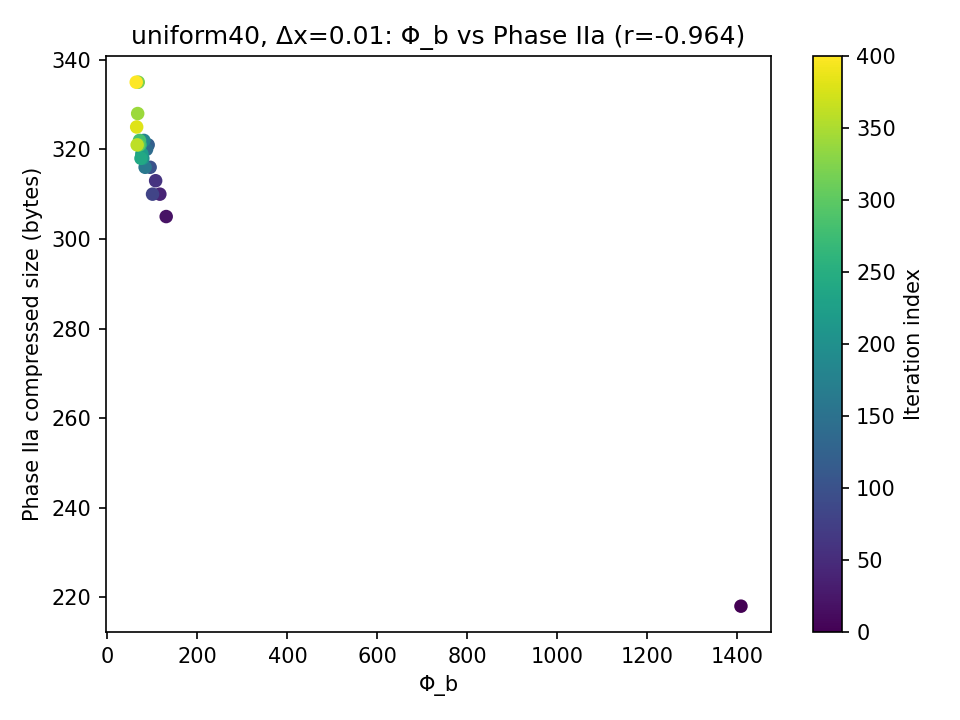
\includegraphics[width=\textwidth]{figures/uniform40_dx0.01_phib_vs_phase2a.png}
\caption{Phase IIa: fixed-order coords (gzip).}
\end{subfigure}\hfill
\begin{subfigure}[b]{0.32\textwidth}
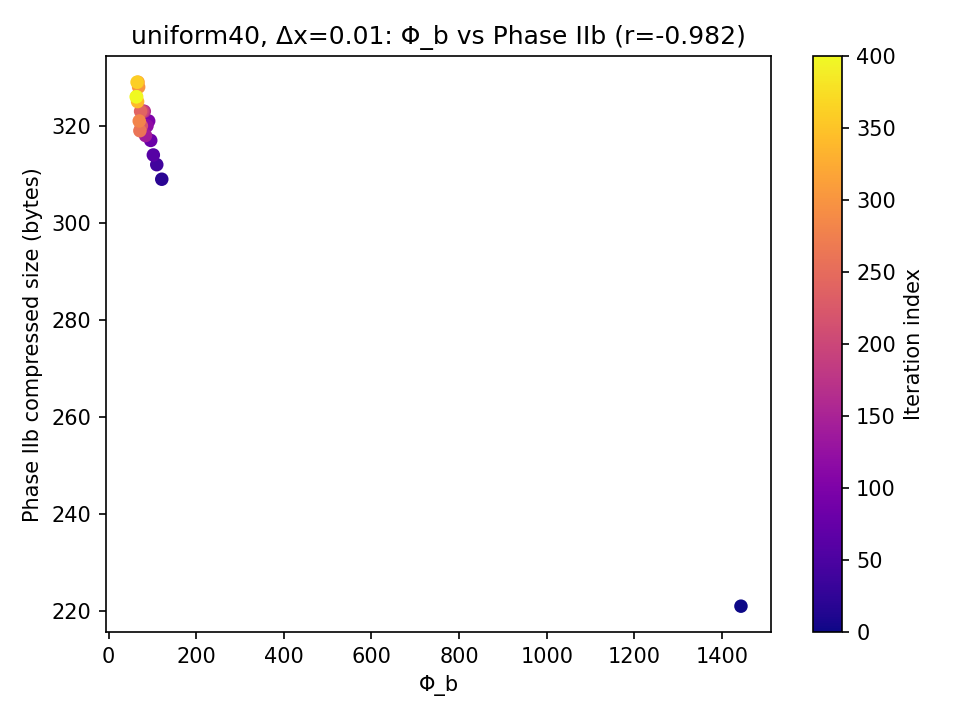
\includegraphics[width=\textwidth]{figures/uniform40_dx0.01_phib_vs_phase2b.png}
\caption{Phase IIb: shuffled-order coords (gzip).}
\end{subfigure}\hfill
\begin{subfigure}[b]{0.32\textwidth}
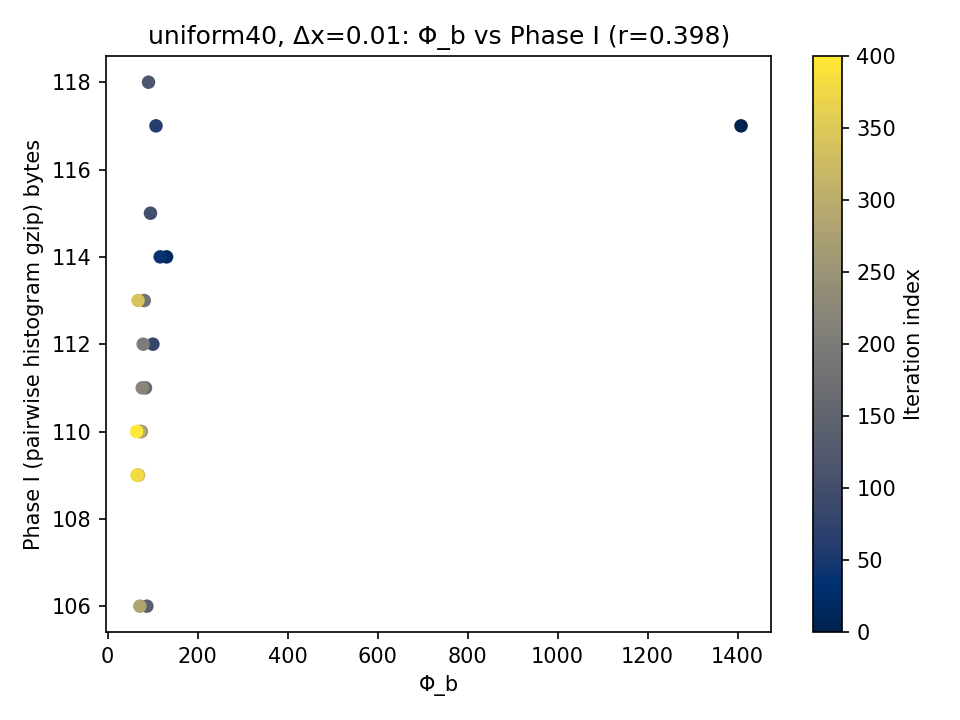
\includegraphics[width=\textwidth]{figures/uniform40_dx0.01_phib_vs_phase1.png}
\caption{Phase I: pair-distance histogram (gzip).}
\end{subfigure}
\caption{\texttt{uniform40}, $\Delta x{=}10^{-2}$. Each point is one subsampled snapshot. Color indicates iteration index (later = darker). Left: Phase IIa shows that $\phib$ predicts compressed size for a coordinate-only encoder. Middle: Phase IIb shows that this survives random shuffling of particle order, addressing ordering artifacts. Right: Phase I shows the internal-consistency relationship between $\phib$ and an explicitly pairwise-distance-based code.}
\label{fig:uniform40_corr}
\end{figure}

\subsection{\texttt{lattice40} ($N{=}40$, $\Delta x = 10^{-2}$)}
\begin{figure}[h!]
\centering
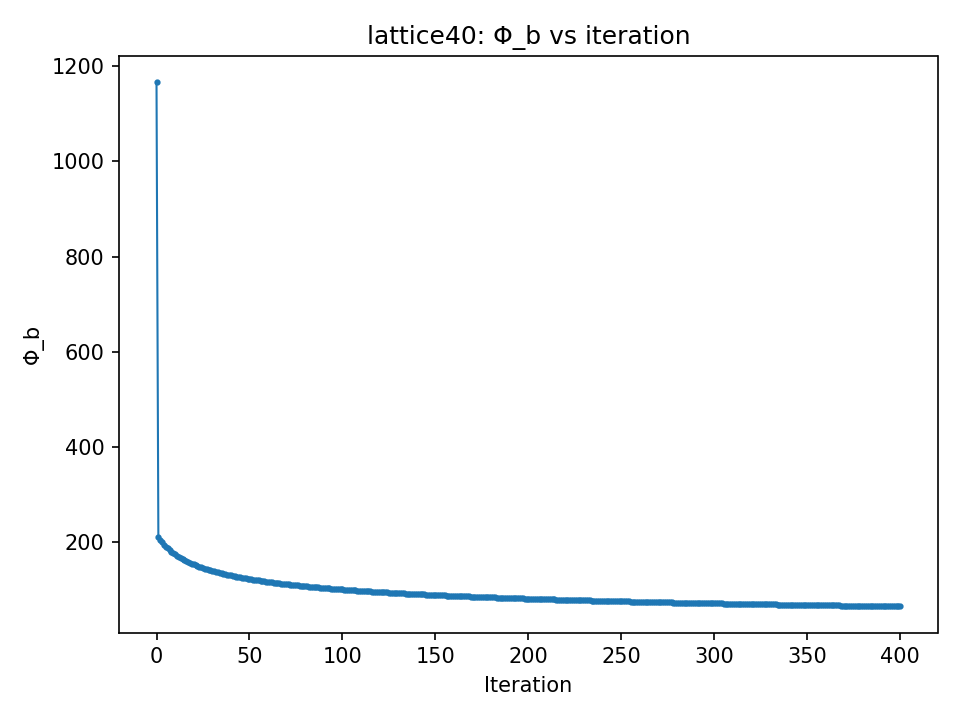
\includegraphics[width=0.6\textwidth]{figures/lattice40_dx0.01_phib_vs_iter.png}
\caption{\texttt{lattice40}. $\phib$ vs iteration. $\phib$ decreases overall but exhibits plateaus and jumps, reflecting limited large-scale rearrangement.}
\label{fig:lattice40_iter}
\end{figure}

\begin{figure}[h!]
\centering
\begin{subfigure}[b]{0.32\textwidth}
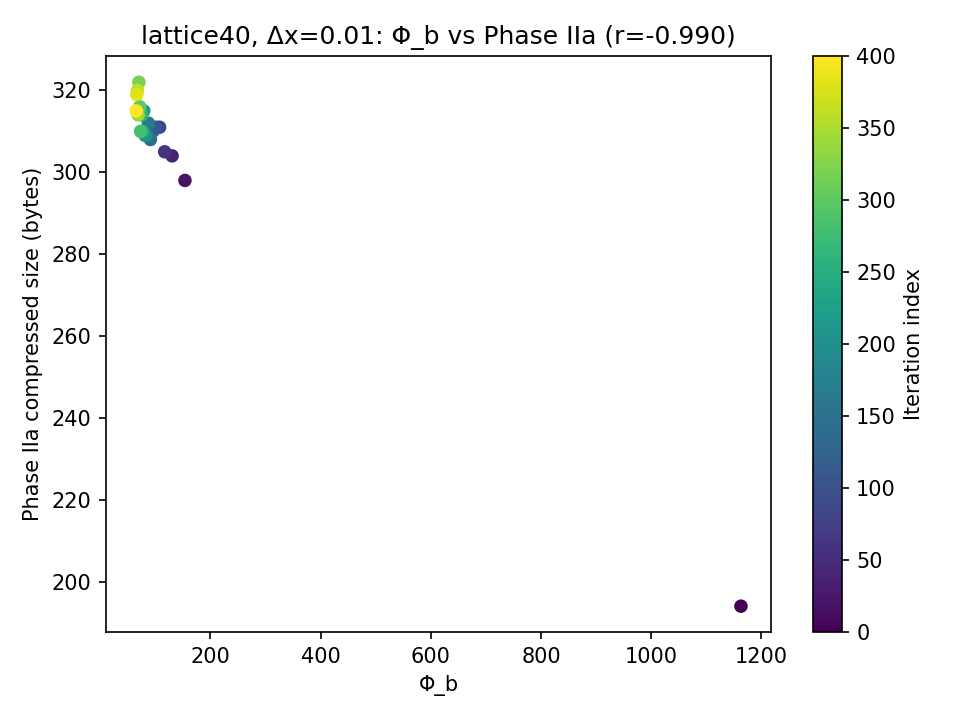
\includegraphics[width=\textwidth]{figures/lattice40_dx0.01_phib_vs_phase2a.png}
\caption{Phase IIa.}
\end{subfigure}\hfill
\begin{subfigure}[b]{0.32\textwidth}
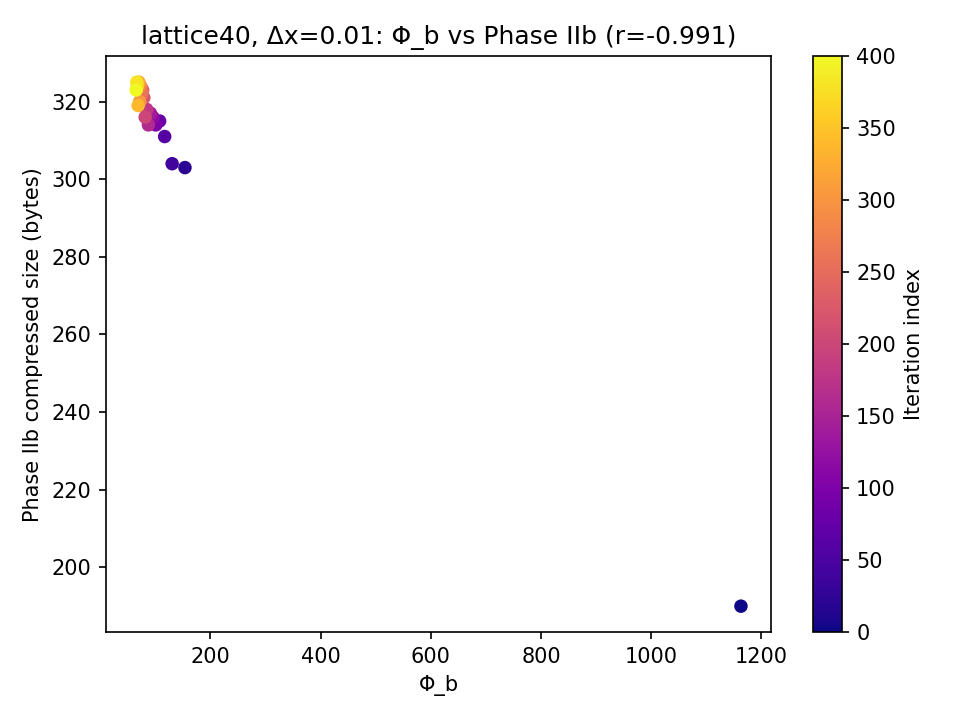
\includegraphics[width=\textwidth]{figures/lattice40_dx0.01_phib_vs_phase2b.png}
\caption{Phase IIb.}
\end{subfigure}\hfill
\begin{subfigure}[b]{0.32\textwidth}
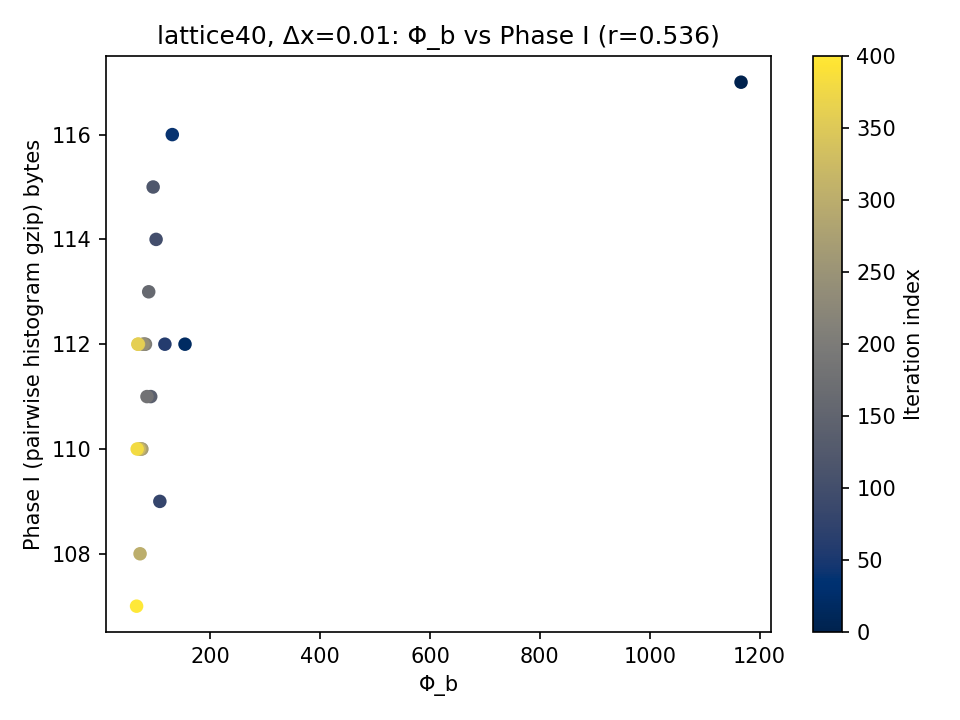
\includegraphics[width=\textwidth]{figures/lattice40_dx0.01_phib_vs_phase1.png}
\caption{Phase I.}
\end{subfigure}
\caption{\texttt{lattice40}, $\Delta x{=}10^{-2}$. Correlations between $\phib$ and compressed size are moderate compared to other ensembles. In some $\Delta x$ settings they fall below the preregistered $|r|\ge0.7$ bar, making \texttt{lattice40} a rejection case under F3. Baseline geometric metrics perform comparably or better, indicating $\phib$ is not uniquely informative for this already structured initial lattice-like configuration.}
\label{fig:lattice40_corr}
\end{figure}

\subsection{\texttt{blobs40} ($N{=}40$, $\Delta x = 10^{-2}$)}
\begin{figure}[h!]
\centering
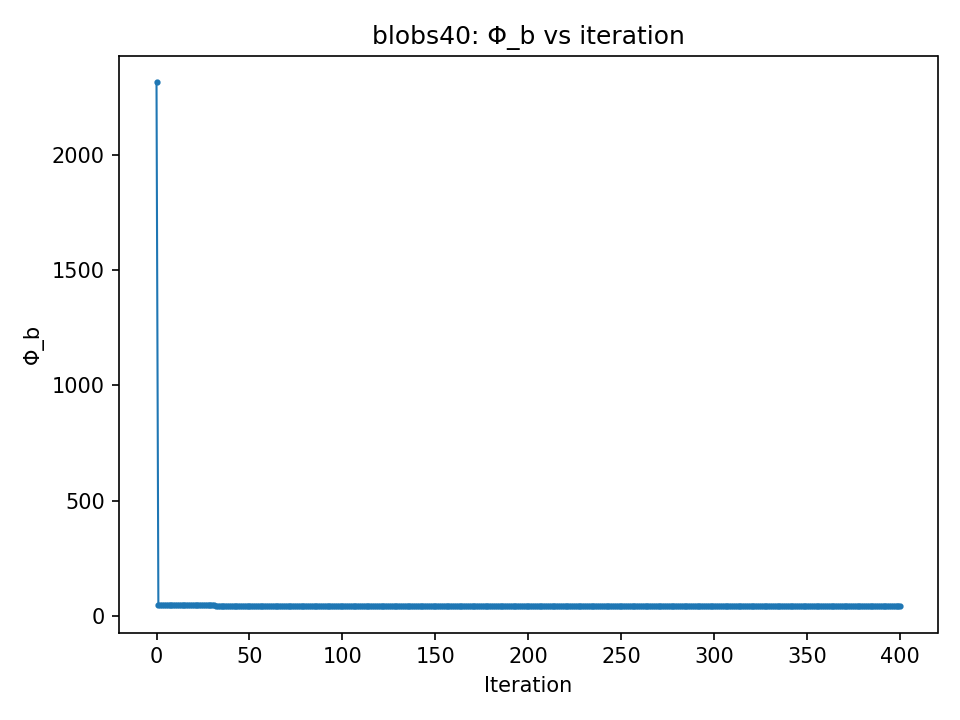
\includegraphics[width=0.6\textwidth]{figures/blobs40_dx0.01_phib_vs_iter.png}
\caption{\texttt{blobs40}. $\phib$ vs iteration, showing monotone reduction under backtracked descent.}
\label{fig:blobs40_iter}
\end{figure}

\begin{figure}[h!]
\centering
\begin{subfigure}[b]{0.32\textwidth}
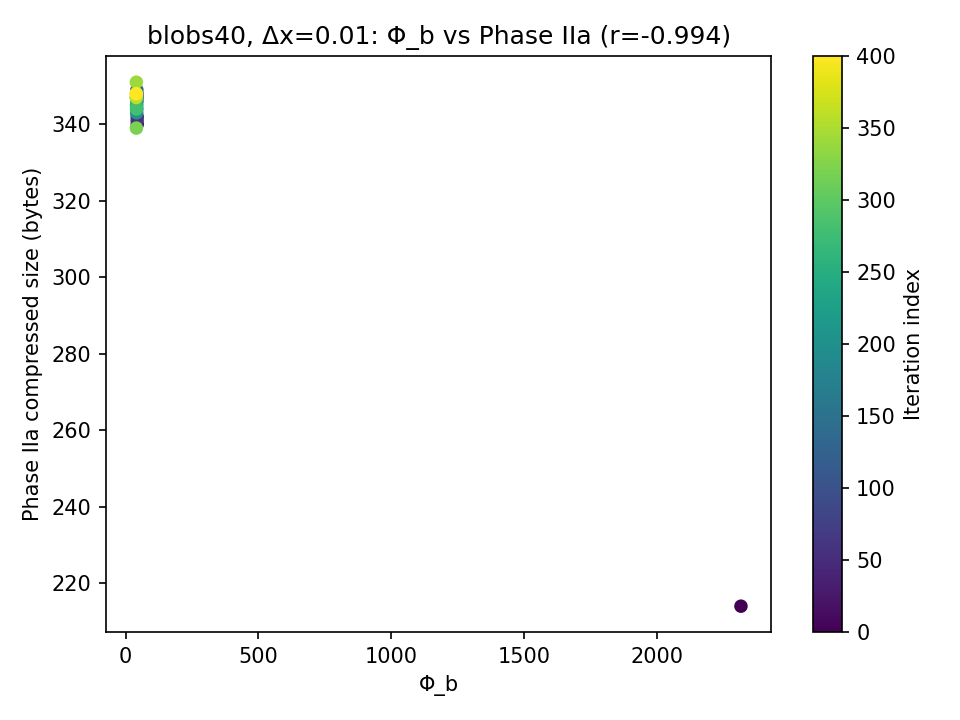
\includegraphics[width=\textwidth]{figures/blobs40_dx0.01_phib_vs_phase2a.png}
\caption{Phase IIa.}
\end{subfigure}\hfill
\begin{subfigure}[b]{0.32\textwidth}
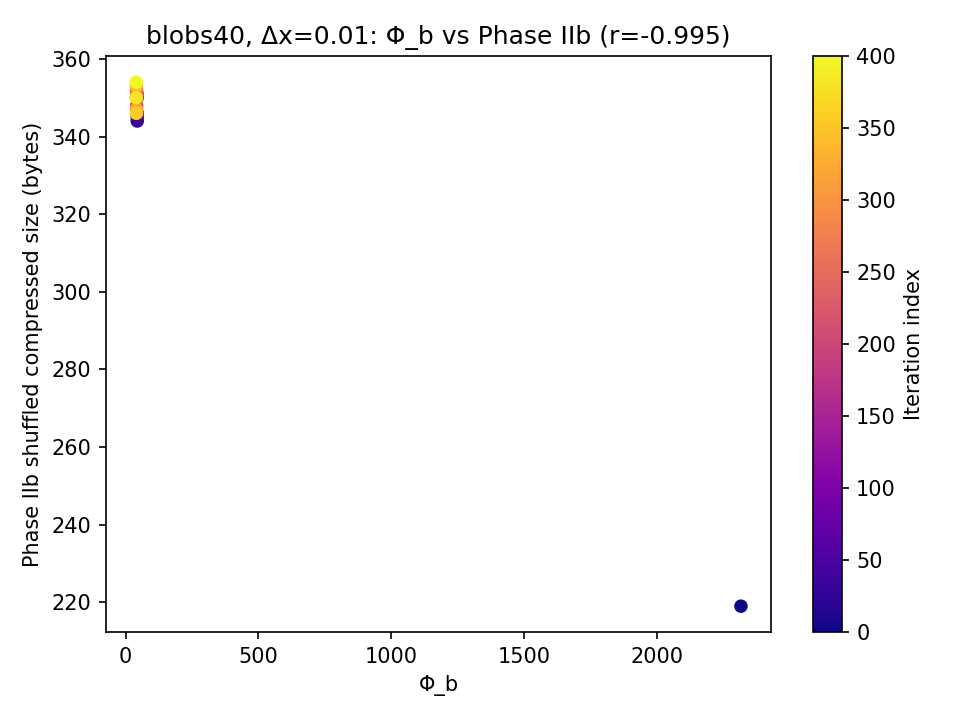
\includegraphics[width=\textwidth]{figures/blobs40_dx0.01_phib_vs_phase2b.png}
\caption{Phase IIb.}
\end{subfigure}\hfill
\begin{subfigure}[b]{0.32\textwidth}
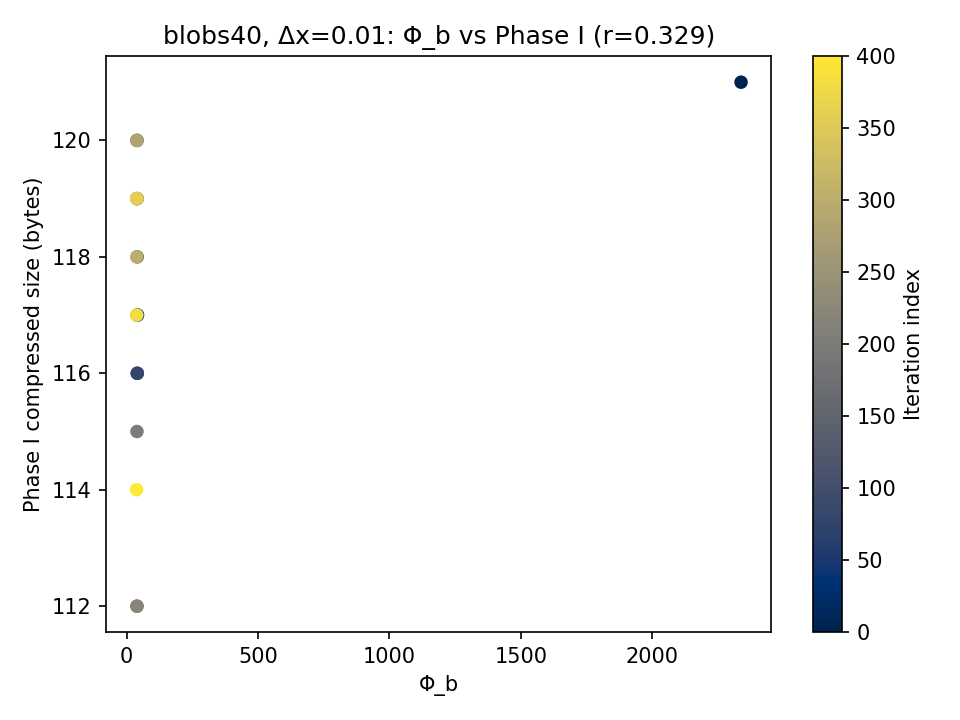
\includegraphics[width=\textwidth]{figures/blobs40_dx0.01_phib_vs_phase1.png}
\caption{Phase I.}
\end{subfigure}
\caption{\texttt{blobs40}, $\Delta x{=}10^{-2}$. Both fixed-order and shuffled-order compressed sizes track $\phib$ with very large $|r|$, and this persists across $\Delta x$. Baseline geometric metrics (e.g.\ mean nearest-neighbor distance) are also strong here, but $\phib$ remains competitive.}
\label{fig:blobs40_corr}
\end{figure}

\subsection{\texttt{uniform400} ($N{=}400$, $\Delta x = 10^{-3}$)}
\begin{figure}[h!]
\centering
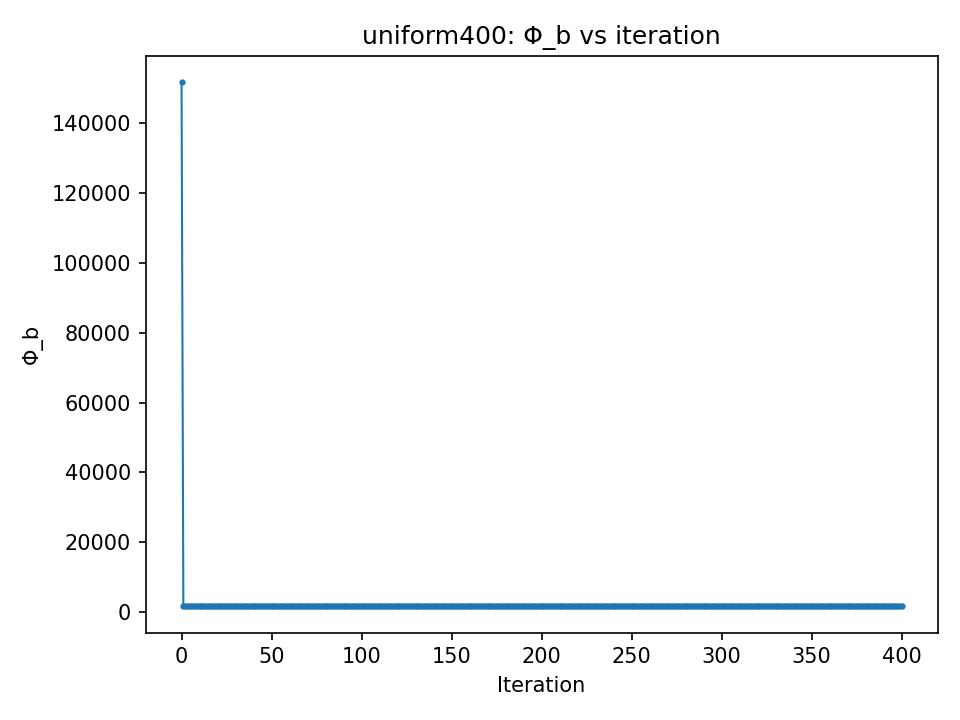
\includegraphics[width=0.6\textwidth]{figures/uniform400_dx0.001_phib_vs_iter.png}
\caption{\texttt{uniform400}. $\phib$ vs iteration. Even at $N{=}400$, backtracking enforces monotone descent.}
\label{fig:uniform400_iter}
\end{figure}

\begin{figure}[h!]
\centering
\begin{subfigure}[b]{0.32\textwidth}
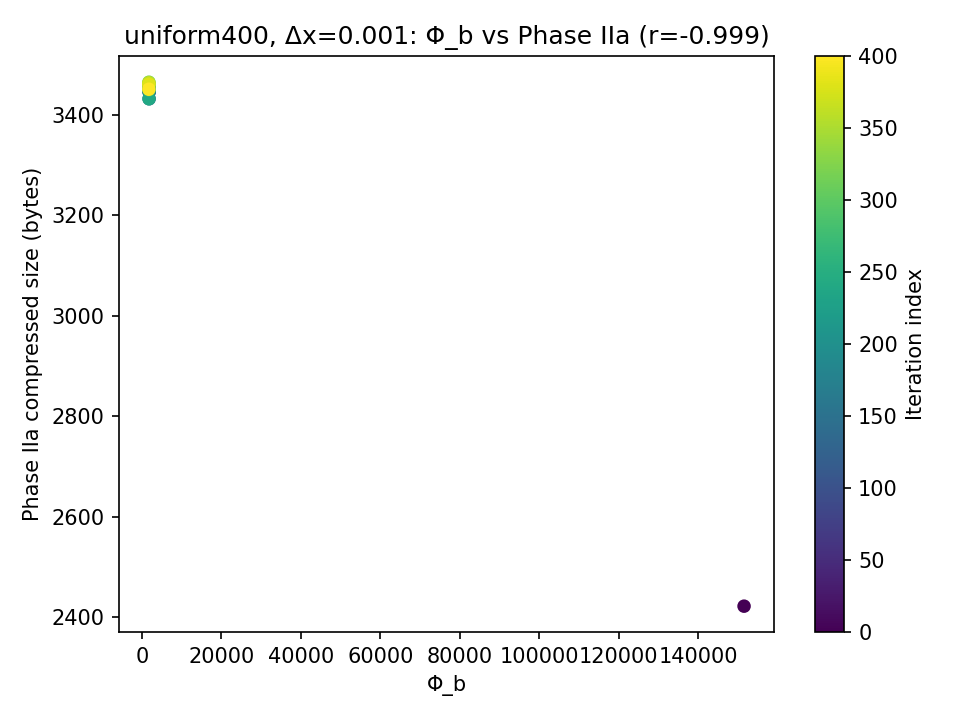
\includegraphics[width=\textwidth]{figures/uniform400_dx0.001_phib_vs_phase2a.png}
\caption{Phase IIa.}
\end{subfigure}\hfill
\begin{subfigure}[b]{0.32\textwidth}
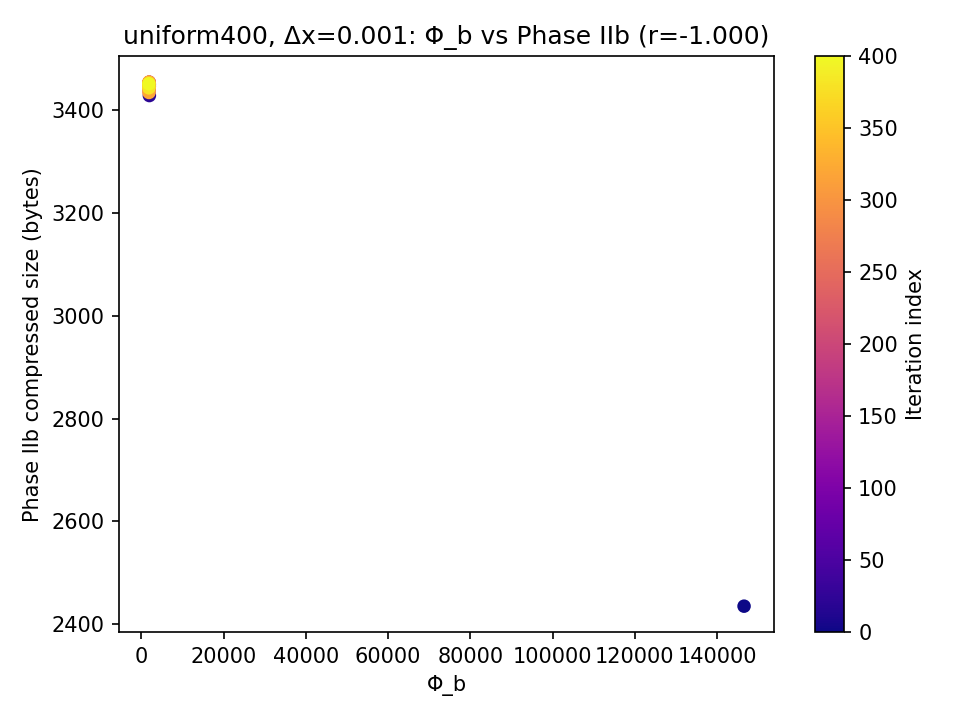
\includegraphics[width=\textwidth]{figures/uniform400_dx0.001_phib_vs_phase2b.png}
\caption{Phase IIb.}
\end{subfigure}\hfill
\begin{subfigure}[b]{0.32\textwidth}
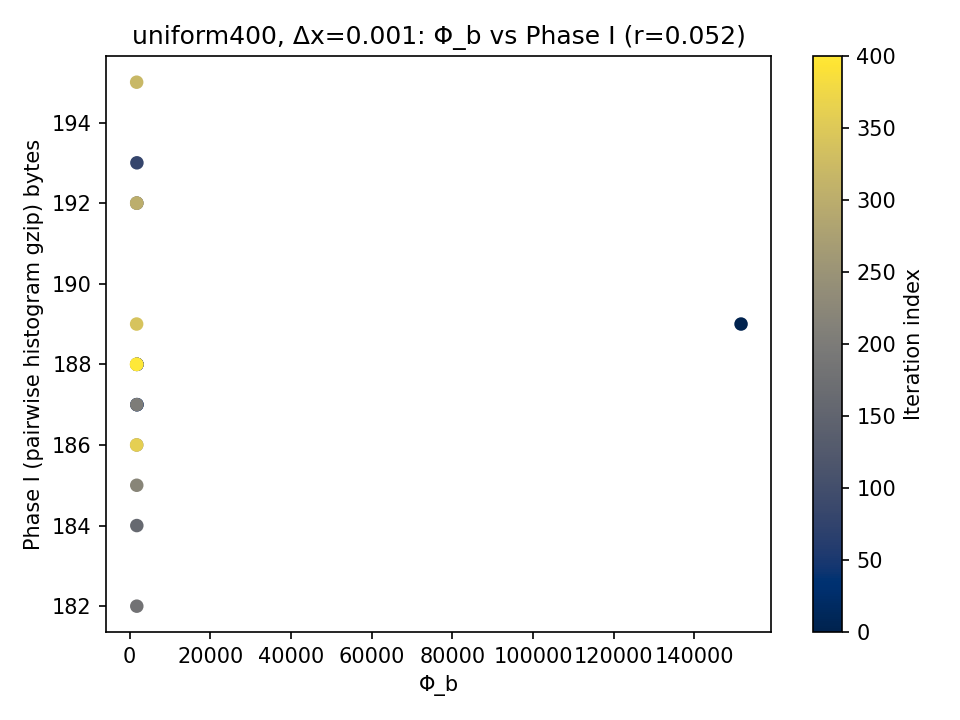
\includegraphics[width=\textwidth]{figures/uniform400_dx0.001_phib_vs_phase1.png}
\caption{Phase I.}
\end{subfigure}
\caption{\texttt{uniform400}, $\Delta x{=}10^{-3}$. $\phib$ and compressed size exhibit an almost perfectly monotonic relationship (Pearson $|r|\approx 1$). This persists after shuffling particle order (Phase IIb), and $\phib$ matches or exceeds naive geometric baselines (radius of gyration, nearest-neighbor distance, coordinate variance).}
\label{fig:uniform400_corr}
\end{figure}

\clearpage

\section{Interpretation}
\subsection{What has been shown}
The experimental loop demonstrates three things.

First, we can \emph{actually run} a specified surrogate $\phib$, evolve systems by explicit descent in $\phib$, and log snapshots and compressed sizes in a way that can either vindicate or kill the surrogate for each ensemble. This answers the demand for preregistered falsifiers that are empirically checkable.

Second, for several ensembles (notably \texttt{uniform40}, \texttt{blobs40}, and especially \texttt{uniform400}), $\phib$ strongly predicts not only a pair-structure-aware ``Phase I'' compressed size, but also a coordinate-only compressed size (Phase IIa). Crucially, this relationship survives in Phase IIb, where we shuffle particle order before compression to break trivial ordering patterns. Phase IIb directly addresses the ``Phase II is not blind'' objection.

Third, not all ensembles behave equally. In \texttt{lattice40}, correlations are weaker and fall below a preregistered $|r|\ge 0.7$ bar for some tested $\Delta x$. We include it anyway and label it a rejection case. This is essential: if the method only ever gave pretty plots, it would not be science.

\subsection{What has \emph{not} been claimed}
We have not claimed:
\begin{itemize}
\item that $\phib$ is unique;
\item that $\phib$ encodes all relevant structure (it is pairwise only; higher-order motifs are not explicitly modeled);
\item that $\phib$ corresponds to any known physical interaction;
\item that the relationship between $\phib$ and compressed size persists in all regimes, ensembles, dimensions, or late times.
\end{itemize}

We explicitly \emph{do not} declare a universal physical law. We present $\phib$ as a computable proxy that can pass or fail an empirical audit.

\subsection{How to read PCD}
The right way to read PCD is:
\begin{enumerate}[label=(\alph*)]
\item \textbf{As a protocol.}  
You propose a computable surrogate for ``compression pressure,'' evolve your system by descending it, and then test whether that surrogate actually predicts independent compression measures. If not, you throw it out for that ensemble.

\item \textbf{As an empirical observation.}  
In several tested ensembles (and more strongly at larger $N$), a specific $\phib$ built purely from local pairwise terms correlates extremely well with how easily full snapshots can be compressed by a generic, external compressor --- even when particle order is randomized before compression, and even across $\Delta x$ values spanning three orders of magnitude.

\item \textbf{As an invitation to extend.}  
You can swap in other surrogates, other encoders (including arithmetic coders or neural compressors), other ensembles, and other ambient dimensions, then repeat. The falsifier (F3) generalizes.
\end{enumerate}

\section{Model Card Template (for preregistration)}
We consider the following information ``preregistered'' for a run:
\begin{itemize}
\item \textbf{System definition.}  
Number of particles $N$, ensemble generator (\texttt{uniform40}, \texttt{lattice40}, \texttt{blobs40}, \texttt{uniform400}, etc.), random seed.

\item \textbf{Surrogate functional.}  
Exact $\phib$ definition (\cref{eq:phib-def}), all hyperparameters (softening $a$).

\item \textbf{Update rule.}  
Gradient descent with backtracking line search, as in \cref{eq:update}, enforcing $\phib$ monotone nonincreasing at accepted steps.

\item \textbf{Snapshot schedule.}  
Save every $k$ accepted steps (e.g.\ every $5$).

\item \textbf{Quantization.}  
Coordinate quantization resolutions $\Delta x \in \{10^{-1},10^{-2},10^{-3}\}$, integer serialization order (fixed vs shuffled for IIa/IIb).

\item \textbf{Encoders.}
  \begin{itemize}
  \item Phase I: pair-distance histogram, histogram bin edges, gzip level (here 6).
  \item Phase IIa: fixed-order coordinate serialization and gzip.
  \item Phase IIb: same, but particle order is permuted uniformly at random before serialization.
  \end{itemize}

\item \textbf{Baselines.}  
Definitions of radius of gyration, mean nearest-neighbor distance, and coordinate variance.

\item \textbf{Falsifier threshold.}  
Required $|r|$ (e.g.\ $0.7$) on decorrelated subsamples of size $n_{\text{eff}}$, with no appeal to classical $p$-values.
\end{itemize}

The intent is: once this card exists, you run the experiment once, report $r$ and $n_{\text{eff}}$ as in \cref{fig:uniform40_iter,fig:uniform40_corr,fig:lattice40_iter,fig:lattice40_corr,fig:blobs40_iter,fig:blobs40_corr,fig:uniform400_iter,fig:uniform400_corr}, and decide: provisionally accept or reject that surrogate \emph{for that ensemble}.

\section{Limitations and Next Steps}
\paragraph{Pairwise-only surrogate.}
$\phib$ only depends on pairwise distances. It will miss higher-order motifs, directional order, chirality, etc. A natural extension is to add local multi-body or patch statistics and rerun the same falsifier pipeline, including Phase IIa/IIb.

\paragraph{Scaling and $N$.}
We tested $N{=}40$ and $N{=}400$. Correlations in Phase II generally become \emph{stronger} at $N{=}400$, suggesting that larger-$N$ structure is being organized in a way that a generic compressor can exploit. We have not yet pushed beyond $N{=}400$; cost profiling will matter.

\paragraph{Autocorrelation / statistics.}
Snapshots along one trajectory are autocorrelated. We partially correct by subsampling snapshots (e.g.\ keep every $20$th) and we report Pearson $r$ and the resulting subsample size $n_{\text{eff}}$. We deliberately do not attach classical $p$-values. A more principled block bootstrap or AR(1)-aware correction is straightforward future work.

\paragraph{Runtime / reproducibility.}
All results here were generated with a single Python script that (i) performs gradient descent with backtracking, (ii) logs snapshots, (iii) runs gzip-based encoders, (iv) computes Pearson $r$, and (v) emits both plots and a summary table. We use a fixed random seed (\texttt{np.random.seed(0)}), a starting step size $\eta_0 \approx 0.05$ with backtracking factor $0.5$, and \texttt{gzip} compression level 6. We evolve for a few hundred accepted steps and subsample every 20th snapshot, giving $n_{\text{eff}}\approx 21$.

\paragraph{Dimensionality and seeds.}
All current tests are in 3D and, for each ensemble type, shown for one representative random draw. Extending to multiple seeds per ensemble and to different ambient dimensions (2D, 10D) is straightforward and is important future work.

\paragraph{Encoders.}
We used gzip for both Phase I (on pair-distance histograms) and Phase IIa/IIb (on raw coordinates). An obvious direction is to try other compressors (arithmetic coders, learned neural compressors) and ask whether $\phib$ still tracks compressed size.

\paragraph{Interpretation of ``falsification.''}
``Falsifier F3'' should be read as: does this surrogate act as a \emph{useful proxy} for compressibility, in this controlled setting, under these encoders? It is not a universal physical statement. When \texttt{lattice40} fails F3, we mark $\phib$ as rejected \emph{for that ensemble}.

\section{Relation to Prior Work}
This work sits at the interface of:
\begin{itemize}
\item \textbf{Gradient flow methods.}  
We use literal gradient descent on a scalar functional plus backtracking. This is standard numerics, but here the scalar is interpreted as ``compression pressure'' and is directly audited against compressed byte size.

\item \textbf{Compression / MDL intuition.}  
The story behind $\phib$ is: ``configurations with more stereotyped pairwise structure can be encoded more concisely.'' The pipeline here is an explicit test of that claim, not just a slogan.

\item \textbf{Force-directed and kernel methods.}  
Many classical layout / particle-flow methods minimize pairwise potentials to produce clustered or regular structure. PCD's novelty is not that such flows exist, but that we insist on testing whether the \emph{same scalar} that drives the flow actually predicts \emph{independent} compression, including after coordinate shuffling.

\item \textbf{Falsifiability / preregistration.}  
We give an explicit falsifier (F3), execute it, and keep runs that ``fail.'' This differs from work that retroactively relabels an energy as ``information'' without a rejection rule.
\end{itemize}

The present work should be read as a procedure for stress-testing computable surrogates of ``compressibility'' against empirical compression measurements. The particle system is a convenient playground for that procedure.

\section{Conclusion}
PCD, as presented here, is a workflow:

\begin{enumerate}[label=(\arabic*)]
\item choose a computable surrogate $\phib$ meant to stand in for ``compression pressure'';
\item evolve a system by monotone descent in $\phib$;
\item measure compressed byte sizes of snapshots under multiple encoders:
  one that explicitly encodes pairwise structure (Phase I),
  one that just gzips quantized coordinates in a fixed order (Phase IIa),
  and one that gzips after shuffling particle order (Phase IIb);
\item sweep quantization scale $\Delta x$ and include naive geometric baselines;
\item compute Pearson $r$ on decorrelated samples and decide, via F3, whether to keep or reject the surrogate for each ensemble.
\end{enumerate}

The experiments reported here show that, for several ensembles (including at $N{=}400$), a simple pairwise-distance surrogate $\phib$ strongly predicts multiple compressed-size measures, including an external coordinate gzip compressor and its shuffled-order control, and in many cases matches or exceeds naive geometric baselines. In other ensembles that link weakens, and we show those too.

That is the core value: the test exists, it is computable, and it sometimes passes. From here, one can iterate: richer surrogates; richer encoders; larger systems; stricter falsifiers.

\section*{Acknowledgments}
We thank colleagues and reviewers for repeatedly insisting on (i) an external encoder that does not bake in pair-distance histograms, (ii) an ordering control (coordinate shuffling), (iii) a quantization sweep, (iv) baseline geometric metrics, (v) temporal subsampling to reduce autocorrelation instead of naive $p$-values, (vi) scaling to larger $N$, and (vii) explicit preregistration of the falsifier.

\bibliographystyle{plain}
\begin{thebibliography}{10}

\bibitem{Shannon1948}
C.~E. Shannon.
\newblock A mathematical theory of communication.
\newblock {\em Bell System Technical Journal}, 27:379--423, 623--656, 1948.

\bibitem{Rissanen1978}
J.~Rissanen.
\newblock Modeling by shortest data description.
\newblock {\em Automatica}, 14(5):465--471, 1978.

\bibitem{LeimkuhlerMatthews2016}
B.~Leimkuhler and C.~Matthews.
\newblock {\em Molecular Dynamics}.
\newblock Springer, 2016.
\newblock (for BAOAB-style splitting integrators and stochastic stability).

\bibitem{Wendland1995}
H.~Wendland.
\newblock Piecewise polynomial, positive definite and compactly supported
  radial functions.
\newblock {\em Adv. Comput. Math.}, 4:389--396, 1995.
\newblock (for smooth compact-support kernels and local interactions).

\bibitem{FruchtermanReingold1991}
T.~M.~J. Fruchterman and E.~M. Reingold.
\newblock Graph drawing by force-directed placement.
\newblock {\em Software: Practice and Experience}, 21(11):1129--1164, 1991.
\newblock (for classical pairwise energy minimization in layouts).

\end{thebibliography}

\end{document}
